% % Side-by-side normalization example (python-pillow/Pillow #6955), color-annotated.
% % Three roles are color-coded in BOTH panels: premises/context (amber), the
% % question/problem statement (blue), and the maintainer's answer (green).
% % Left: the raw mined thread, reproduced verbatim (CVE list and multi-comment
% % triage abbreviated) -- the question (c6) asks about "the remaining three,"
% % a dangling reference that only resolves against the earlier triage.
% % Right: the normalized item. Focus is solely on the transformation.

% % role colors (light backgrounds, mid-tone borders, dark text for labels)
\definecolor{cAsk}{RGB}{255,246,224}\definecolor{bAsk}{RGB}{226,176,84}\definecolor{tAsk}{RGB}{150,90,10}
\definecolor{cPrem}{RGB}{232,240,254}\definecolor{bPrem}{RGB}{120,160,230}\definecolor{tPrem}{RGB}{28,70,170}
\definecolor{cAns}{RGB}{231,248,238}\definecolor{bAns}{RGB}{108,190,150}\definecolor{tAns}{RGB}{20,118,70}

% % one normalized block: label + tinted, bordered minipage with body
% \long\def\normblock#1#2#3#4#5{% {bg}{border}{labelcolor}{label}{body}
%   \fcolorbox{#2}{#1}{\begin{minipage}{\dimexpr\linewidth-2\fboxsep\relax}\footnotesize
%   {\scriptsize\bfseries\color{#3}#4}\\[2pt]#5\end{minipage}}}

% \begin{figure*}[t]
% \centering
% \setlength{\fboxsep}{6pt}
% %================ (a) raw mined thread ================
% \begin{minipage}[t]{0.485\textwidth}
% {\small\textbf{(a) Raw mined thread}}\;\;{\scriptsize\itshape python-pillow/Pillow \#6955, as posted (abbreviated)}\\[3pt]
% \begin{lstlisting}[style=rawthread,frame=tlr,rulecolor=\color{black!35},backgroundcolor=\color{cPrem},aboveskip=0pt,belowskip=0pt,xleftmargin=4pt,xrightmargin=4pt,framexleftmargin=4pt,framexrightmargin=4pt]
% TITLE: Libtiff vulnerabilities (CVE-2022-2519, CVE-2022-2520, CVE-2022-48281)

% [c0  crbean | reporter]
% Some libtiff vulnerabilities in Pillow -- please
% confirm whether you are affected:
%  ~CVE-2022-2056~ ~CVE-2022-2057~ CVE-2022-2519
%  CVE-2022-2520 ~CVE-2022-2521~ ... CVE-2022-48281
% OS: Linux   Python: 3.9   Pillow: 9.3.0
% \end{lstlisting}
% \begin{lstlisting}[style=rawthread,frame=lr,rulecolor=\color{black!35},backgroundcolor=\color{cPrem},aboveskip=0pt,belowskip=0pt,xleftmargin=4pt,xrightmargin=4pt,framexleftmargin=4pt,framexrightmargin=4pt]
% [c1-c4  hugovk | maintainer]
% Several are already handled in #6577, #6681,
% #6746 (not affected). Most of the rest relate to
% tiffcrop, which we don't use. "To summarise,
% Pillow is not affected by any of these; please
% search the issue tracker next time."
% \end{lstlisting}
% \begin{lstlisting}[style=rawthread,frame=lr,rulecolor=\color{black!35},backgroundcolor=\color{cAsk},aboveskip=0pt,belowskip=0pt,xleftmargin=4pt,xrightmargin=4pt,framexleftmargin=4pt,framexrightmargin=4pt]
% [c5/c6  crbean | reporter]
% The previous issue was on 9.2.0; not sure about
% 9.3.0. Excuse me, are the remaining three
% affected? CVE-2022-2519, CVE-2022-2520,
% CVE-2022-48281
% \end{lstlisting}
% \begin{lstlisting}[style=rawthread,frame=blr,rulecolor=\color{black!35},backgroundcolor=\color{cAns},aboveskip=0pt,belowskip=0pt,xleftmargin=4pt,xrightmargin=4pt,framexleftmargin=4pt,framexrightmargin=4pt]
% [c7  hugovk | maintainer]
% Pillow is not affected: these are related to
% tiffcrop, which we don't use. Same for
% CVE-2022-2520.
% \end{lstlisting}
% \end{minipage}
% \hfill
% %================ (b) normalized evaluation item ================
% \begin{minipage}[t]{0.495\textwidth}
% {\small\textbf{(b) Normalized evaluation item}}\;\;{\scriptsize\itshape self-contained}\\[3pt]
% \normblock{cPrem}{bPrem}{tPrem}{PREMISES / CONTEXT}{%
% A scanner flags several libtiff CVEs against Pillow~\texttt{9.3.0} (Linux, Python~3.9). After the maintainer triaged the list, three remained in question: CVE-2022-2519, CVE-2022-2520, and CVE-2022-48281.}

% \smallskip
% \normblock{cAsk}{bAsk}{tAsk}{QUESTION}{%
% Is Pillow~\texttt{9.3.0} affected by these three libtiff vulnerabilities---CVE-2022-2519, CVE-2022-2520, and CVE-2022-48281?}

% \smallskip
% \normblock{cAns}{bAns}{tAns}{GOLD ANSWER}{%
% No---Pillow is not affected by any of the three. They are vulnerabilities in libtiff's \texttt{tiffcrop} tool, which Pillow does not use.}
% \end{minipage}

% \smallskip
% {\centering\footnotesize\setlength{\fboxsep}{2.5pt}%
% \fcolorbox{bPrem}{cPrem}{\rule{0pt}{1.4ex}\rule{1.4ex}{0pt}}~premises / context \quad
% \fcolorbox{bAsk}{cAsk}{\rule{0pt}{1.4ex}\rule{1.4ex}{0pt}}~question / problem statement \quad
% \fcolorbox{bAns}{cAns}{\rule{0pt}{1.4ex}\rule{1.4ex}{0pt}}~answer\par}

% \caption{\textbf{Normalization turns a verified thread into a gradeable item}
% (\texttt{python-pillow/Pillow}~\#6955; \S\ref{sec:normalization}). Color marks the
% three roles in both panels: \colorbox{cPrem}{premises / context}, the
% \colorbox{cAsk}{question / problem statement}, and the \colorbox{cAns}{answer}.
% \textbf{(a)}~As mined, the pair is not gradeable as-is: the reporter dumps a long
% list of libtiff CVEs, the maintainer triages them across four comments, and only
% then does the reporter ask the real question (\texttt{c6})---which leans on that
% exchange, ``are the \emph{remaining three} affected?'', a dangling reference whose
% meaning depends on the preceding triage.
% \textbf{(b)}~A single LLM pass, then human-verified, makes the question
% self-contained: it resolves ``the remaining three'' to the explicit CVE
% identifiers and inlines the premises the answer needs (the affected package and
% versions), leaving one crisp question, and it distills the maintainer's reply into
% a faithful gold answer that adds no claim the thread does not make. The CVE
% triage, the cross-issue references, and the housekeeping (``please search the
% tracker'') are dropped. The CVE list is abbreviated for space.}
% \label{fig:normalization}
% \end{figure*}


\begin{figure}
    \centering
    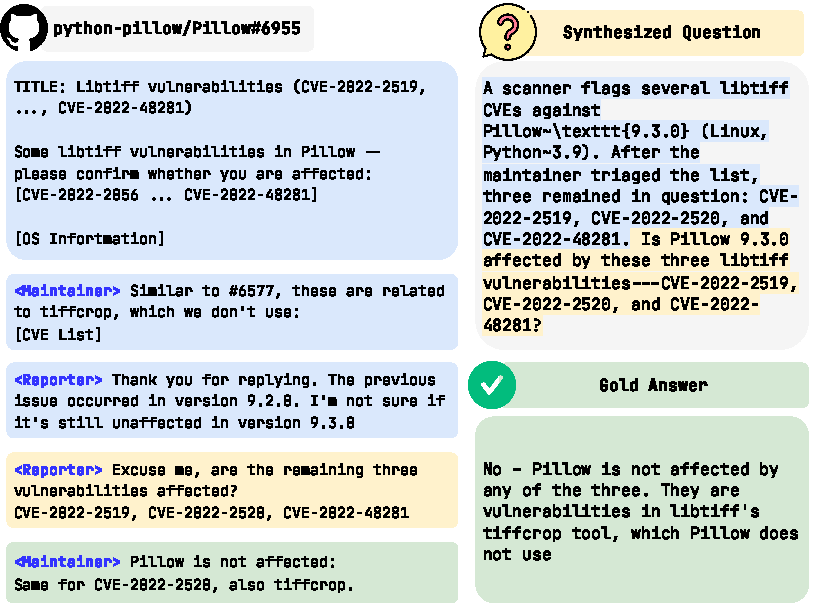
\includegraphics[width=\linewidth]{figures/secdevqa-normalization.pdf}
    \caption{QA synthesis turns a verified thread into a gradeable item
(\texttt{python-pillow/Pillow}~\#6955; \S\ref{sec:normalization}). Color marks the
three roles in both panels: \colorbox{cPrem}{premises / context}, the
\colorbox{cAsk}{question / problem statement}, and the \colorbox{cAns}{answer}.}
\label{fig:normalization}
\end{figure}